\section{Theorie}

    Im folgenden Abschnitt sollen die theoretischen Grundlagen der Bestimmung der Suszeptibilität aus atomaren Größen
    sowie der experimentellen Messung aufgeführt werden.

\subsection{Die paramagnetische Suszeptibilität}

    Die Suszeptibilität $\chi$ ist ein Faktor,
    der temperaturabhängig ist
    und Einfluss auf die magnetische Flussdichte $\symbf{B}$ in Materie hat.
    \begin{equation*}
        \symbf{B} = \mu_0 \symbf{H} + \symbf{M}
    \end{equation*}
    Die Größe $\symbf{M}$ stellt die Magnetisierung dar,
    um die sich das Magnetfeld in Materie im Vergleich zum Vakuum unterscheidet.
    Es gilt
    \begin{equation}
        \label{eqn:Magnetisierung}
        \symbf{M} = \mu_0 \chi \symbf{H} .
    \end{equation}
    \\
    Im Gegensatz zum Diamagnetismus,
    welcher eine allgemeine Eigenschaft von Materie ist und auf Induktion magnetischer Momente gründet,
    ist der Paramagnetismus nur bei Atomen, Ionen oder Molekülen zu finden,
    die einen nicht-verschwindenen Drehimpuls besitzen,
    da sich die magnetischen Momente relativ zum äußeren Magnetfeld orientieren.
    Beim Diamagnetismus verschwindet der Drehimpuls durch die entgegengesetzte Orientierung der magnetischen Momente
    im äußeren und induzierten Magnetfeld.
    Der Paramagnetismus ist zudem temperaturabhängig,
    da sich die magnetischen Momente,
    welche eine Auswirkung auf den Drehimpuls haben,
    durch die thermische Bewegung der Materie umorientieren.\\
    Der Gesamtdrehimpuls $\symbf{J}$ eines Atoms setzt sich aus dem Bahndrehimpuls der Elektronenhülle,
    dem Eigendrehimpuls, also dem Spin der Elektronen und dem Kerndrehimpuls,
    welcher hier allerdings vernachlässigt werden kann,
    zusammen.\\
    Es gilt die \enquote{LS-Kopplung}
    \begin{equation*}
        \symbf{J} = \symbf{L} + \symbf{S} ,
    \end{equation*}
    mit dem Gesamtbahndrehimpuls $\symbf{L}$, der durch
    \begin{equation*}
        \symbf{L} = \sum \symbf{l}_\text{i}
    \end{equation*}
    definiert ist,
    und dem Gesamtspin $\symbf{S}$, der durch
    \begin{equation*}
        \symbf{S} = \sum \symbf{s}_\text{i}
    \end{equation*}
    definiert ist.
    Die zugehörigen magnetischen Momente sind
    \begin{align*}
        \symbf{\mu_\text{L}} &= - \frac{\mu_\text{B}}{\hbar} \symbf{L} \\
        \symbf{\mu_\text{S}} &= - g_\text{S} \frac{\mu_\text{B}}{\hbar} \symbf{S}
    \end{align*}
    mit dem Bohr'schen Magneton $\mu_\text{B} = \frac{1}{2} \frac{\symup{e}_0}{\symup{m}_0} \hbar$.
    Der Faktor $g_\text{S}$ stellt das gyromagnetische Verhältnis des freien Elektrons dar.
    Die zugehörigen Beträge der Impulse sind durch
    \begin{align*}
        \lvert \symbf{L} \rvert &= \sqrt{L(L+1)} \cdot \hbar \\
        \lvert \symbf{S} \rvert &= \sqrt{S(S+1)} \cdot \hbar \\
        \lvert \symbf{J} \rvert &= \sqrt{J(J+1)} \cdot \hbar
    \end{align*}
    gegeben,
    mit der Bahndrehimpulsquantenzahl $L$,
    der Spinquantenzahl $S$ und der Gesamtbahndrehimpulsquantenzahl $J$. \\
    Die Beträge der magnetischen Momente sind durch
    \begin{align*}
        \lvert \symbf{\mu_\text{L}} \rvert &= \mu_\text{B} \sqrt{L(L+1)} \\
        \lvert \symbf{\mu_\text{S}} \rvert &= \mu_\text{B} \sqrt{S(S+1)}
    \end{align*}
    gegeben. \\
    Für die LS-Kopplung gilt,
    dass nur die parallele,
    beziehungsweise die antiparalle Komponente $\symbf{\mu_\text{J}}$ zu $\symbf{J}$ messbar ist.
    Mit der Winkelbeziehung
    \begin{equation*}
        \lvert \symbf{\mu_\text{J}} \rvert = \lvert \symbf{\mu_\text{S}} \rvert cos(\alpha) + \lvert \symbf{\mu_\text{L}} \rvert cos(\beta)
    \end{equation*}
    lässt sich der Landé-Faktor des Atoms herleiten.
    Er wird durch
    \begin{equation}
        \label{eqn:Lande_Faktor}
        g_\text{J} = \frac{3J(J+1) + (S(S+1) - L(L+1))}{2J(J+1)}
    \end{equation}
    beschrieben mit der Vereinfachung $g_\text{S} = 2$.\\
    Der Landé-Faktor kann mithilfe der Hund'schen Regeln berechnet werden:
    \begin{enumerate}
        \label{Hundsche_Regeln}
        \item Der Gesamtspin $\symbf{S}$ wird aus den einzelnen Spins $\symbf{s}_\text{i}$ zusammengesetzt,
        die nach dem Pauli-Prinzip möglich sind.
        \item Der Gesamtdrehimpuls $\symbf{L}$ wird aus den einzelnen Bahndrehimpulsen $\symbf{l}_\text{i}$ zusammengesetzt,
        die nach dem Pauli-Prinzip möglich sind.
        \item Der Gesamtdrehimpuls $\symbf{J}$ wird durch $\symbf{J} = \symbf{L} - \symbf{S}$ beschrieben,
        wenn eine Schale weniger als zur Hälfte gefüllt ist,
        und durch $\symbf{J} = \symbf{L} + \symbf{S}$,
        wenn eine Schale mehr als zur Hälfte gefüllt ist.
    \end{enumerate}
    Für die hier zu untersuchenden Ionen Seltener Erden wurde beobachtet,
    dass sie besonders stark paramagnetisch sind,
    da die Atomhüllen große Drehimpulse
    – gerade in den inneren Schalen –
    besitzen.
    Der Grund dafür sind die Elektronen in der nicht ganz gefüllten 4f-Schale.
    Elemente mit dieser Eigenschaft sind im Periodensystem erst ab der dritten Hauptgruppe (z=58) zu finden.
    Die vorherigen Schalen sind vollständig gefüllt,
    sodass es dort zu einem verschwindenen Drehimpuls kommt.\\
    \\
    Zusätzlich ist die Richtungsquantelung für die Berechnung der Suszeptibilität relevant.
    Sie bestimmt,
    dass nur Winkel,
    bei denen die Komponente $\mu_{\text{J}_\text{z}}$ ein Vielfaches von $\mu_\text{B} g_\text{J}$ ist,
    also
    \begin{equation*}
        \mu_{\text{J}_\text{z}} = \mu_\text{B} g_\text{J} \cdot m ,
    \end{equation*}
    zwischen der Richtung des äußeren Magnetfeldes und der Ausrichtung von $\symbf{\mu_\text{J}}$ möglich sind.
    Die Zahl $m$ ist dabei die Orientierungsquantenzahl.
    Sie ist ganzzahlig und bewirkt,
    dass es nur $2J+1$ Einstellmöglichkeiten der Ausrichtung zwischen äußerem Magnetfeld und magnetischen Moment gibt.
    Die zu den $2J+1$ Einstellmöglichkeiten gehörige potentielle Energie ist durch
    \begin{equation*}
        E_\text{m} = - \symbf{\mu_\text{J}} \cdot \symbf{B} = \mu_{\text{J}_\text{z}} B = \mu_\text{B} g_\text{J} \cdot m B
    \end{equation*} %Ich bin mir nicht sicher, ob in der Anleitung bei (15) ein Fehler bei der Formatierung ist
    gegeben und beschreibt die Energie beim Paramagnetismus.\\
    Für die magnetische Suszeptibilität ergibt sich nach Einsetzen und Umformen der \autoref{eqn:Magnetisierung}
    \begin{equation}
        \label{eqn:chi_T}
        \chi = \frac{\mu_0 {\mu_\text{B}}^2 {g_\text{J}}^2 N J (J+1)}{3kT}
    \end{equation}
    mit der Boltzmann-Konstante $k$ und der Temperatur $T$.
    Für hinreichend hohe Temperaturen gilt nach dem Curie'schen Gesetz des Paramagnetismus
    \begin{equation*}
        \chi \propto \frac{1}{T} \ .
    \end{equation*}

\subsection{Experimentelle Bestimmung der paramagnetischen Suszeptibilität}
    Aus in \autoref{sec:theorie:störspannungen} erläuterten Gründen wird
    für die Messung der Suszeptibilität eine Brückenschaltung verwendet.

    \begin{figure}
      \centering
      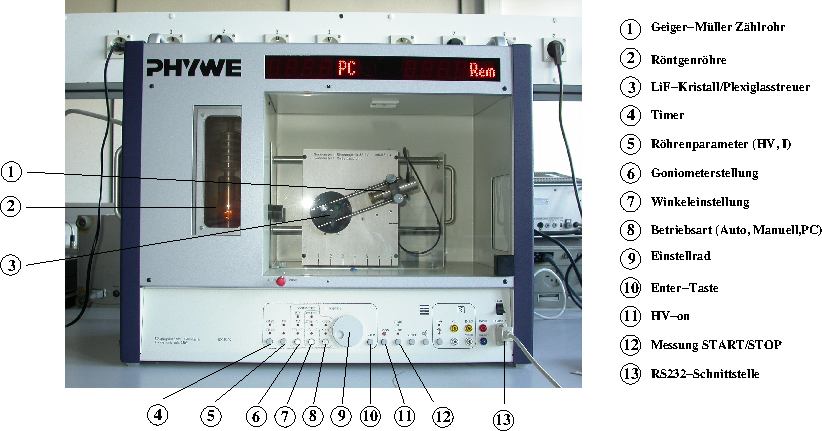
\includegraphics[width=0.5\textwidth]{content/img/Abb_2.pdf}
      \caption{Schaltplan der verwendeten Brückenschaltung. \cite{versuchsanleitung}}
      \label{fig:Brückenschaltung}
    \end{figure}
    Mithilfe dieser Brückenschaltung sollen die Induktivitäten zweier etwa gleich langer Spulen gemessen werden,
    wobei eine der Spulen eine Probe von Seltener Erde enthält.\\
    Für die Induktivität der Spule in Materie gilt
    \begin{equation*}
        L_\text{M} = \mu_0 \frac{n^2 F}{l} + \chi \mu_0 \frac{n^2 Q}{l} ,
    \end{equation*}
    wobei $n$ die Windungszahl, $l$ die Länge, $F$ der Querschnitt der Spule und $Q$ der Querschnitt der Probe ist.
    Für den Unterschied der Induktivitäten in Vakuum $L = \mu_0 \frac{n^2 F}{l}$ und in Materie ergibt sich
    \begin{equation*}
        \symup{\Delta} L = \mu_0 \chi Q \frac{n^2}{l} .
    \end{equation*}
    Das Grundprinzip der Messung mit einer Brückenschaltung besteht darin,
    die Brücke ohne eine Probe abzugleichen und die Brückenspannung und den zu variierenden Widerstand zu messen,
    dann eine Probe einzufügen und die Brücke erneut abzugleichen.
    Die Suszeptibilität kann aus den Änderungen der Spannung oder des Widerstands berechnet werden.\\
    Für die Widerstände,
    die in \autoref{fig:Brückenschaltung} gezeigt sind, gilt
    \begin{align*}
        r_1 &= R_\text{M} + i \omega L_\text{M} \\
        \frac{1}{r_2} &= \frac{1}{R_\text{P}} + \frac{1}{R + i \omega L} \\
        r_3 &= R_3 \\
        r_4 &= R_4 .
        %Wir haben glaube ich immer sofort R3/R4 gemessen oder?
    \end{align*}
    Die Widerstände $R$ und $R_\text{M}$ sind Verlustwiderstände der Spulen.
    Zudem ist $R_3 \approx R_4$.
    Für die Brückenspannung in einer Brückenschaltung mit eingefügter Probe gilt
    \begin{equation*}
        U_\text{Br} = \frac{r_4 r_1 - r_3 r_2}{(r_1 + r_2)(r_3 + r_4)} U_\text{Sp}
        %Was ist U_Sp?
    \end{equation*}
    und nach Einsetzen der Widerstände und Induktivitäten aus den obigen Gleichungen ergibt sich für den Betrag der Brückenspannung
    \begin{equation*}
        \lvert U_\text{Br} \rvert = \frac{\omega \mu_0 \chi n^2 Q}{4l} \frac{1}{\sqrt{R^2 + {\omega}^2(\mu_0 \frac{n^2}{l}F)^2}} \lvert U_\text{Sp} \rvert
    \end{equation*}
    und damit wiederum die Suszeptibilität $\chi$
    \begin{equation}
        \label{eqn:SusU}
        \chi = \frac{\lvert U_\text{Br} \rvert}{\lvert U_\text{Sp} \rvert} \frac{4l}{\omega \mu_0 n^2 Q} \sqrt{R^2 + {\omega}^2(\mu_0 \frac{n^2}{l}F)^2} \ .
    \end{equation}
    Für die Brückenschaltung ohne eingefügte Probe gilt die Abgleichbedingung
    \begin{equation*}
        r_1 R_4 = r_2 R_3 .
    \end{equation*}
    Nachdem die Probe eingefügt wurde,
    ändert sich der Widerstand $R_3$ zu $R'_3 = R_3 + \symup{\Delta}R$ .
    Für die Änderung ergibt sich nach Einsetzen der Gleichungen für die Widerstände in die Abgleichbedingung
    \begin{equation*}
        \symup{\Delta}R = \frac{R_3 (L_\text{M} - L)}{L + L_\text{M}} .
    \end{equation*}
    Nach Einsetzen von $L$ und $L_\text{M}$ kann die Suszeptibilität $\chi$ durch
    \begin{equation}
        \label{eqn:SusR}
        \chi = 2 \frac{\symup{\Delta}R}{R_3} \frac{F}{Q}
    \end{equation}
    berechnet werden.

\subsection{Unterdrückung von Störspannungen}
\label{sec:theorie:störspannungen}

    Eine Schwierigkeit bei der Messung der Brückenspannung besteht darin,
    dass an den Ausgangsklemmen der Schaltung Störspannungen entstehen,
    welche einen breiten Frequenzbereich abdecken.
    Um die monofrequente Brückenspannung zu messen,
    kann daher ein Bandpassfilter verwendet werden,
    welcher nur für einen schmalen Frequenzbereich durchlässig ist.
    Mithilfe eines Selektivverstärkers,
    welcher eine Filterkurve in Gestalt einer Glockenfunktion besitzt,
    wird derselbe Effekt erzielt.

    \begin{figure}
      \centering
      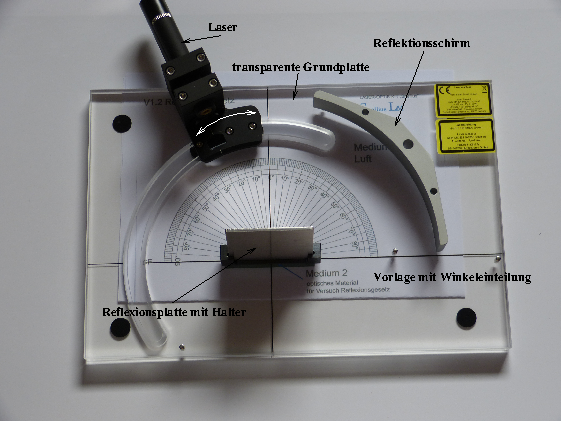
\includegraphics[width=0.5\textwidth]{content/img/Abb_3.pdf}
      \caption{Filterkurve eines Selektivverstärkers. \cite{versuchsanleitung}}
      \label{fig:Filterkurve}
    \end{figure}

    \autoref{fig:Filterkurve} stellt das Verhältnis der Ausgangspannung $U_\text{A}$ zur Eingangsspannung $U_\text{E}$ in Abhängigkeit der Frequenz $\nu$ dar.\\
    Die Güte $Q$ kann (ähnlich wie die Breite der Kurve) als ein Maß für die Wirksamkeit gesehen werden.
    Sie wird mithilfe der Gleichung
    \begin{equation}
        \label{eqn:güte}
        Q = \frac{\nu_0}{\nu_+ - \nu_-}
    \end{equation}
    berechnet.
    Die Frequenz $\nu_0$ stellt die Durchlassfrequenz dar
    und $\nu_+$ und $\nu_-$ die Frequenzen,
    bei denen $\frac{U_\text{A}}{U_\text{E}}$ unter einen Wert von $\frac{1}{\sqrt{2}}$ fällt.\\
    Aufgrund der endlichen Güte können Störspannungen in einem gewissen Frequenzbereich um $\nu_0$ weiterhin durch den Filter gelangen.
